\chapter{基本维护和安全防护}
\label{cha:basic-maintenance}

\begin{intro}
  上一章我们认识到了「网络世界的险恶」——恶意软件层出不穷、安装捆绑无处不在。在这样的环境之下,掌握电脑的简单维护方法、学习如何保护自己的安全,就显得尤为重要了。阅读完这章的内容,你将找到下面这些问题的答案:
  \begin{itemize}
    \item 不小心安装了不想要的软件,怎么卸载它们?
    \item 为什么打开有些软件时,系统总是提示「你要允许此应用对你的设备进行更改吗」?
    \item 杀毒软件?安全中心?电脑管家?到底用什么?
    \item 为什么电脑天天都在「更新」?
    \item 网络上不干净的东西这么多,我要怎么才能「洁身自好」?
  \end{itemize}
\end{intro}

掌握一定的电脑维护的方法,例如软件的卸载、恶意软件的排查,以及了解一些电脑的安全维护的策略和措施,是保障我们「网上冲浪」安全的重要一环。在这一章,我们将了解一些常用的电脑维护技巧,以及一些电脑安全方面的常识。

\section{软件的卸载}

上一章我们介绍了软件的寻找与安装,这里我们就来介绍软件的卸载。软件的安装需要通过安装包来进行,而软件的卸载则是安装的逆过程,除了删除软件自身的文件之外,还会撤销一些写入系统的修改,解除一些文件关联等。因此,软件的卸载也需要通过软件自身提供的卸载工具进行,不是找到安装目录把所有文件全部删除了事,更不是直接删除桌面上的图标(快捷方式)。

在 Windows 11 系统上,一般的软件卸载可以按下面的步骤进行:

\begin{itemize}
  \item 打开系统设置。
  \item 在界面左侧点击【应用】,然后在右侧选择【安装的应用】(部分版本称【应用和功能】),如\autoref{fig:Applications_11}。
  \item 等待右侧下方的列表加载完成。这个列表就是你的电脑上安装的所有软件。找到你不想要的软件,点击这一行右侧的【\makebox[.8em]{⁝}】,再点击【卸载】,如\autoref{fig:Uninstall_an_app_11}。
    \begin{figure}[htb!]
      \centering
      \begin{minipage}{.49\textwidth}
        \centering
        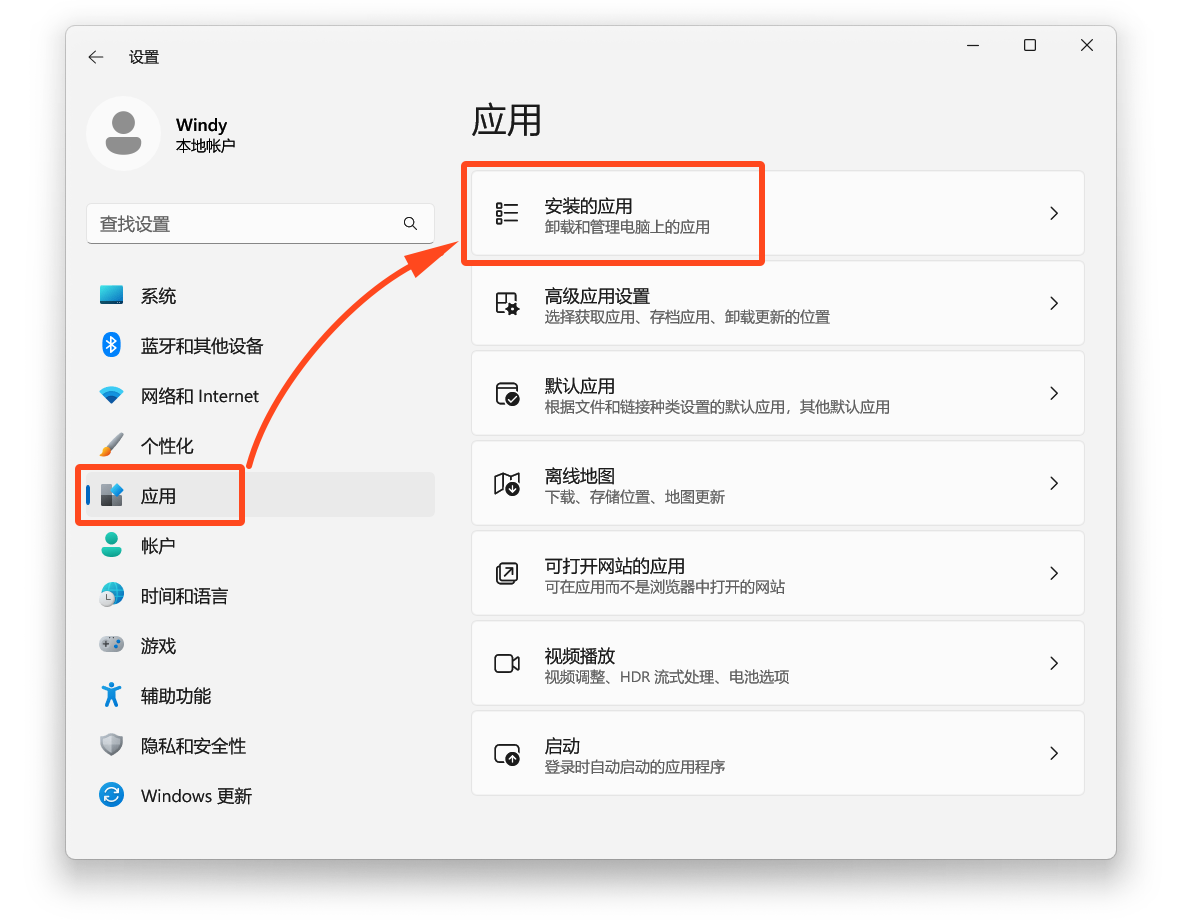
\includegraphics[width=\textwidth]{assets/basic/Applications_11.png}
        \caption{打开 Windows 11 中的应用列表}
        \label{fig:Applications_11}
      \end{minipage}
        \begin{minipage}{.49\textwidth}
        \centering
        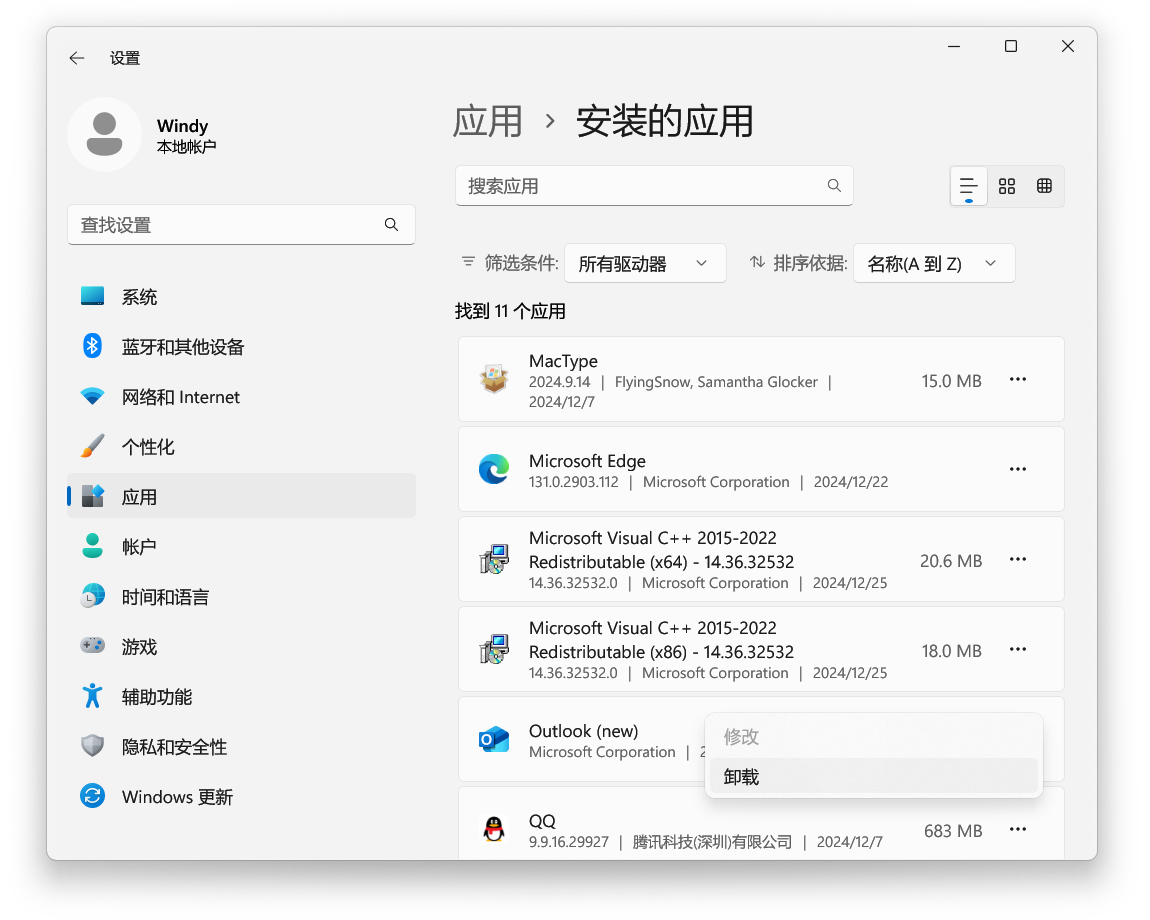
\includegraphics[width=\textwidth]{assets/basic/Uninstall_an_app_11.png}
        \caption{在 Windows 11 中卸载应用}
        \label{fig:Uninstall_an_app_11}
    \end{minipage}
    \end{figure}
  \item 之后根据提示卸载即可。
\end{itemize}

而在 Windows 10 上则是这样:

\begin{itemize}
  \item 打开系统设置。
  \item 选择【应用】,如\autoref{fig:Applications_10}。
  \item 稍等片刻以使得列表完全加载。在这个界面上,会列出电脑中安装的所有软件。找到我们不想要的软件,然后点击两次【卸载】,如\autoref{fig:Uninstalling_an_app_10}。
  \begin{figure}[htb!]
    \centering
    \begin{minipage}{.44\textwidth}
      \centering
      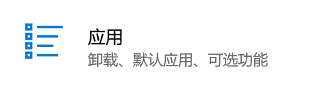
\includegraphics[width=.8\textwidth]{assets/basic/Applications_10.png}
      \caption{打开 Windows 10 中的应用列表}
      \label{fig:Applications_10}
    \end{minipage}
    \begin{minipage}{.55\textwidth}
      \centering
      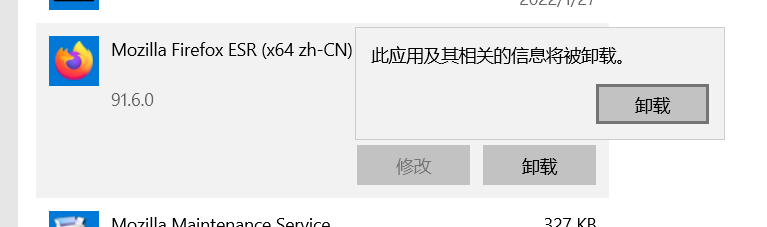
\includegraphics[width=.9\textwidth]{assets/basic/Uninstalling_an_app_10.png}
      \caption{在 Windows 10 中卸载应用}
      \label{fig:Uninstalling_an_app_10}
    \end{minipage}
  \end{figure}
  \item 根据提示进行卸载操作即可。
\end{itemize}

一般来说,卸载很快就能完成。但需要特别注意的是,一些软件的卸载界面错综复杂,\regcolor{充斥有大量的无关选项}(例如【再想想】【我要重装】),因此在点选时务必十分小心。\regcolor{甚至有些软件在卸载完成后会诱导用户装一个新的其他软件,请千万注意。}例如:

\begin{figure}[htb!]
  \centering
  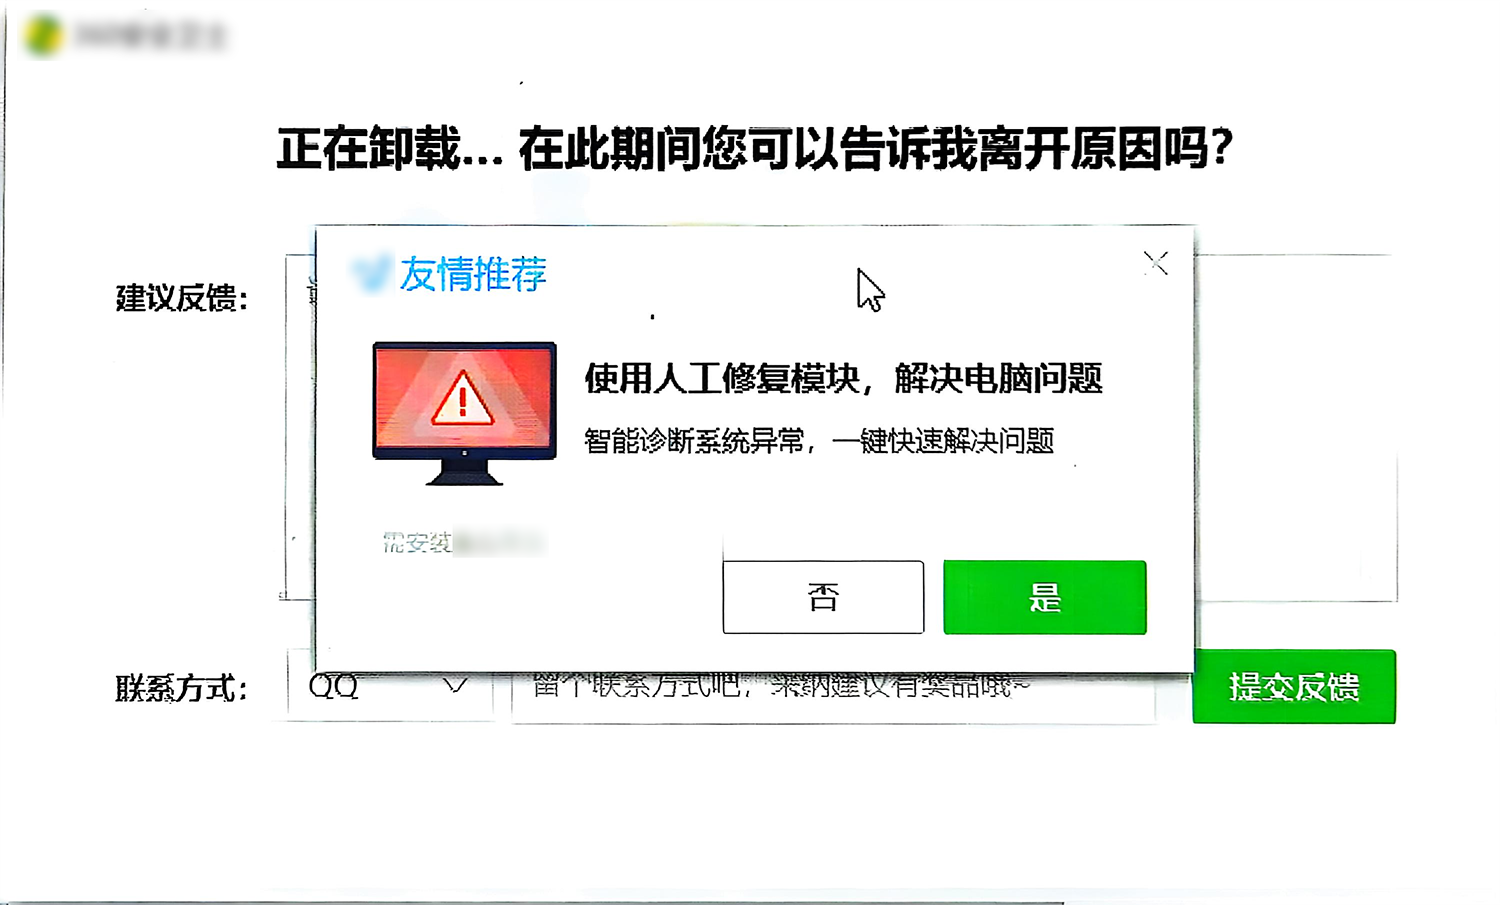
\includegraphics[width=.6\textwidth]{assets/basic/Recommending_others_during_uninstallation.png}
  \caption{诱导安装}
  \label{Confusing_Uninstall}
\end{figure}

有的软件可能会在卸载完成后,提示你需要重启电脑来进行一些最后的清理工作。通常,我们可以选择立即重启;如果你手头还正需要使用电脑,也可以在合适的时候手动重启。

\section{应用的权限与 UAC 弹窗}

这一节我们简单介绍 Windows 系统中的权限机制\footnote{如果你在使用中压根没见过\autoref{fig:UAC_popup} 这样的窗口(即 UAC 弹窗),那么这一节的内容对你可能不适用。你可以去 \chapref{cha:user-and-ms-account}一章了解更多信息。}。在 Windows 系统中,一个程序在一开始启动时仅被赋予了有限的权限——它不能更改系统的一些关键设置,不能在系统中安装新的软件,不可以动一些关键数据。对于大多数程序来说,这些权限就够用了:一般的程序也不会去动那些系统级的设置或者给你装一个什么新软件。它们只需要安分守己地读写自己的文件,帮助用户完成工作就可以了。

但是,在一些特殊的情况下,这种有限的权限对程序来说会变得不够用。例如:

\begin{itemize}
  \item 对于\regcolor{安装包}来说,安装包本身的工作就是安装新的软件,而有限的权限禁止了这种行为。
  \item 对于一些\regcolor{专业软件}来说,它需要连接到一些系统级的部件才能工作,而有限的权限禁止了这种行为。
  \item 对于一些\regcolor{「系统优化」类的软件}来说,它本身就是需要更改系统设置的,而有限的权限禁止了这种行为。
\end{itemize}

\begin{wrapfigure}[12]{r}{6.5cm}
  \centering
  % \vspace*{-.5cm}
  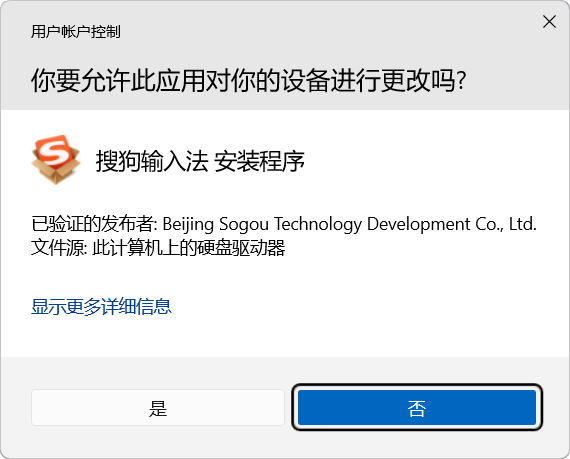
\includegraphics[width=6cm]{assets/basic/UAC_popup.png}
  \caption{一个 UAC 弹窗}
  \label{fig:UAC_popup}
\end{wrapfigure}

此时,程序需要提升自己的权限来完成自己的工作,这个过程称为「提权」。而右图展示的这种弹窗(「你要允许此应用对你的设备进行更改吗」,称为「UAC 弹窗」),则是程序在向系统申请提权时,系统对用户的提示。这样就能解释,为什么在大多数安装或者卸载软件的时候,系统都会弹出这个窗口询问我们;而只有我们点击【是】,安装或者卸载才能正常继续了。

那么这种 UAC 弹窗的意义是什么呢?想象一下这个场景:你电脑上的某个垃圾软件留下的「种子」正在蠢蠢欲动,想要给你电脑安装一套恶意软件。然而,默认情况下,这枚「种子」没有足够的权限,因此它邪恶的计划就这样直接被粉碎了——没有提升的权限,它就没有办法进行软件安装。这也告诉了我们一个重要的事实:\regcolor{如果电脑弹出了不明的 UAC 弹窗,请一律拒绝}

一般来说,「提权」这件事是软件自行向系统申请的。但是有一些软件设计时考虑不周全,它不会自行向系统申请提权,但它正常工作又必须有提升的权限。对于这样的软件,我们可以在启动它时点击右键,选择【以管理员身份运行】,在 UAC 弹窗中选择【是】,就可以手动赋予这个软件提升的权限了。或许你会在使用中发现,一些老旧的软件在安装时就常常需要这么做。

当然,这一套权限系统是有很多空子的。提升的权限具有从属关系——如果某个程序被提权,那么由它打开的其他程序也默认具有特权。因而,如果你为一个不怀好意的程序赋予了特权,那它就可以为所欲为了,因为它能够不动声色地给其他程序特权,然后做一些不好的事情。所以,最终我们还是需要控制住自己电脑上软件的来源,不要让「不干净」的软件来到我们的电脑上。因此,\regcolor{不运行来源不明的可执行文件},是保证安全的根本。

\section{合理使用杀毒软件和安全软件}

合理使用各种杀毒软件、安全软件(后文统称「安全软件」)可以保护你的电脑安全,然而若运用得不合理,也会极大影响我们使用电脑的体验。今天,市面上有大量优秀的国内外安全软件供我们选择——例如,国产的「360 安全卫士」「火绒安全软件」「瑞星杀毒软件」,以及国外的「卡巴斯基」「诺顿」等。同时,Windows 操作系统亦内置了一款「Windows 安全中心」(旧称「Windows Defender」),它也提供了强大的病毒防护和安全保护等功能,如下图所示。这里,我们不具体地推荐某一款安全软件,而是会向你介绍一些相对合理地使用这类软件的方法。

\begin{figure}[htb!]
  \centering
  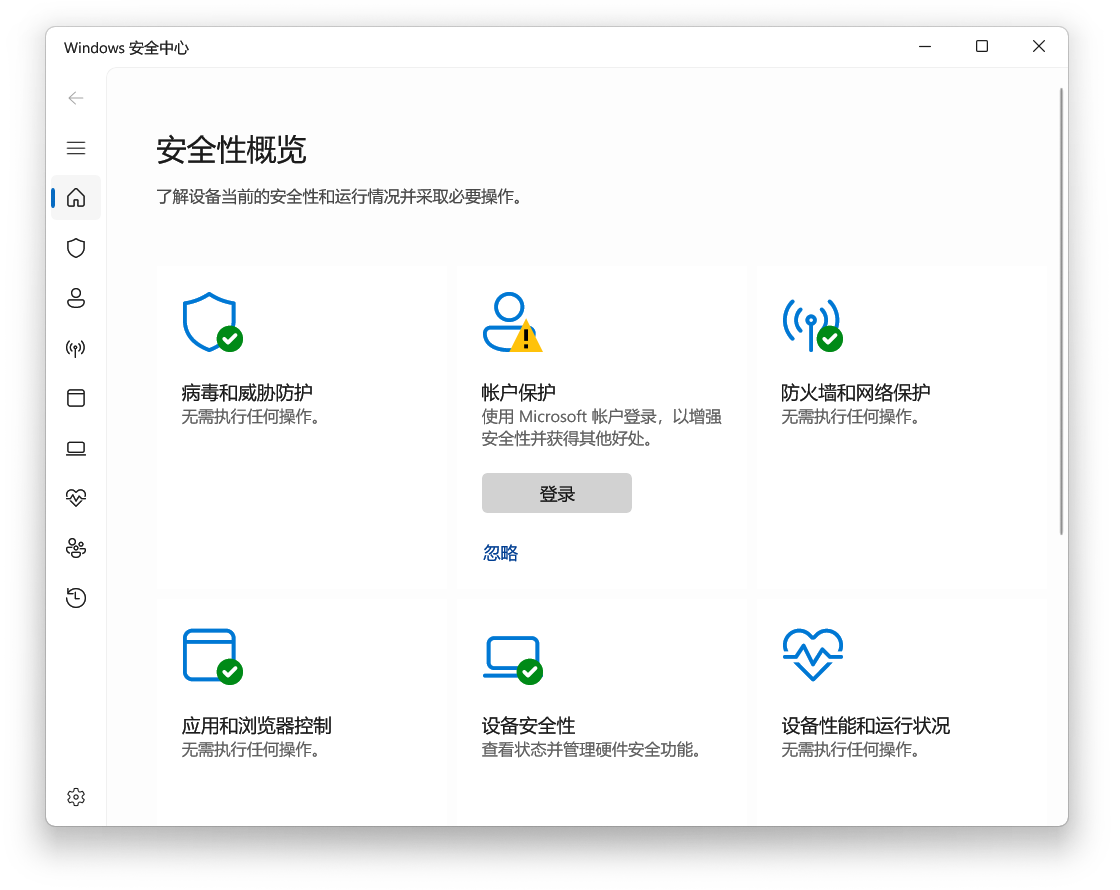
\includegraphics[width=.64\textwidth]{assets/basic/Windows_Security.png}
  \caption{Windows 安全中心}
  \label{fig:Windows_Security}
\end{figure}

首先,\regcolor{永远不要在电脑上同时安装多于一个杀毒软件}。例如,安装了「360 安全卫士」或者「360 杀毒」,就不要再安装「火绒安全软件」或者「腾讯电脑管家」。如果你同时安装多个安全软件,不仅没有必要,它们之间还会因权限冲突而互相「攻击」\CJKsout*{(这就是养蛊)}。

\regcolor{当心「全家桶」。}大型软件厂商都会希望用户能选择自己的整套产品系列。以「腾讯电脑管家」为例,它会以各种方式推荐用户安装包括但不限于「QQ 浏览器」「QQ 游戏」「腾讯桌面整理」等一整套腾讯产品。但事实上,很多时候,我们只是希望安装一款安全软件或杀毒软件来保护我们的电脑罢了。稍不留神,这些软件就会因为某个隐秘的角落的勾勾没有去掉,而来到我们的电脑上。

\begin{figure}[htb!]
  \centering
  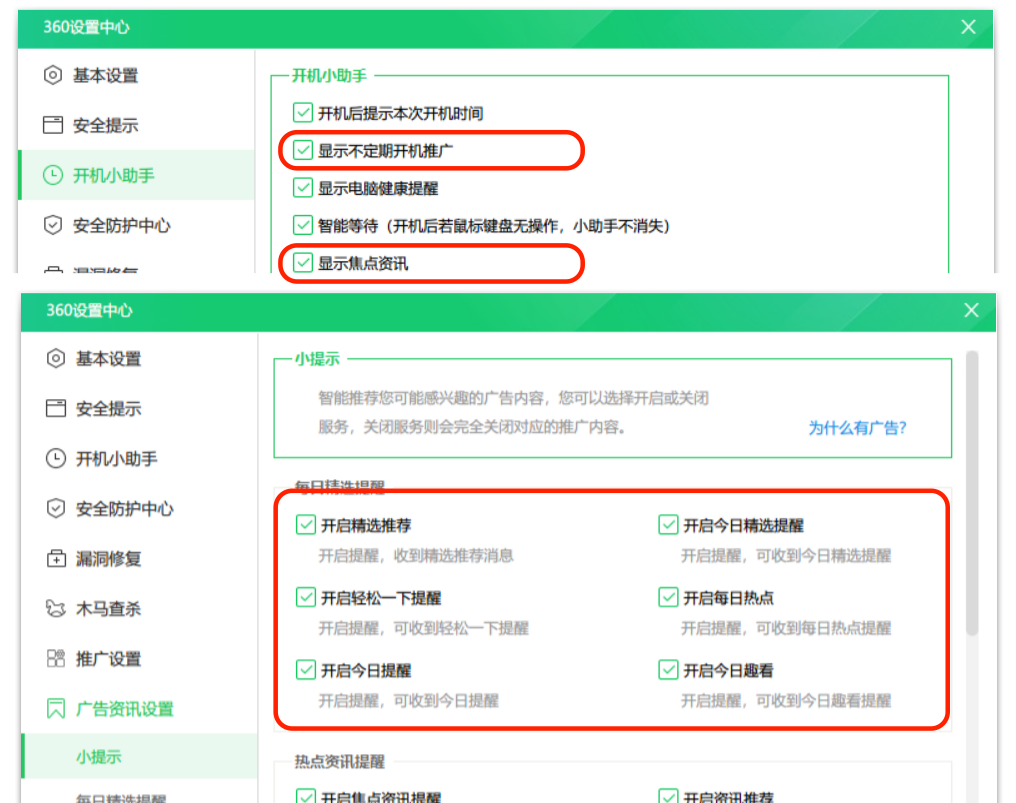
\includegraphics[width=.64\textwidth]{assets/basic/Disable_360_ads.png}
  \caption{360 安全卫士的一些设置项}
  \label{fig:Disable_360_ads}
\end{figure}

我们安装安全软件是为了保障电脑安全,而不是希望这些软件来拖慢我们电脑的运行速度。因此,它们需要经受一些「调教」,才能更好地为我们服务。具体地说,我们可以\regcolor{关闭那些无用的功能和提示},例如每次开机时的启动时间提示、桌面上碍事的「一键加速」加速球、各种「资讯」弹窗广告和「猜你喜欢」搜索框等。这些东西与安全毫不相关,反而有些喧宾夺主。将它们关闭,可以让我们的电脑更加清爽,也不会影响到安全软件的正常工作。以「360 安全卫士」为例,我们可以在软件设置的【开机小助手】【推广设置】【广告资讯设置】等页面中,关闭我们不需要的功能,如\autoref{fig:Disable_360_ads} 所示。

\section{Windows 更新——让人又爱又恨的「更新」}

Windows 一直在不断的更新之中——这里的「更新」指的不是诸如「Windows 7」「Windows 10」这样的大版本的更新,而是那时不时阻碍我们关机睡觉的「Windows 更新」。打开系统设置,Windows 10 选择【更新与安全】(下左图)、Windows 11 选择【Windows 更新】(下右图),你就能看到现在可用的一些 Windows 更新以及它们的状态。

\begin{figure}[htb!]
  \centering
  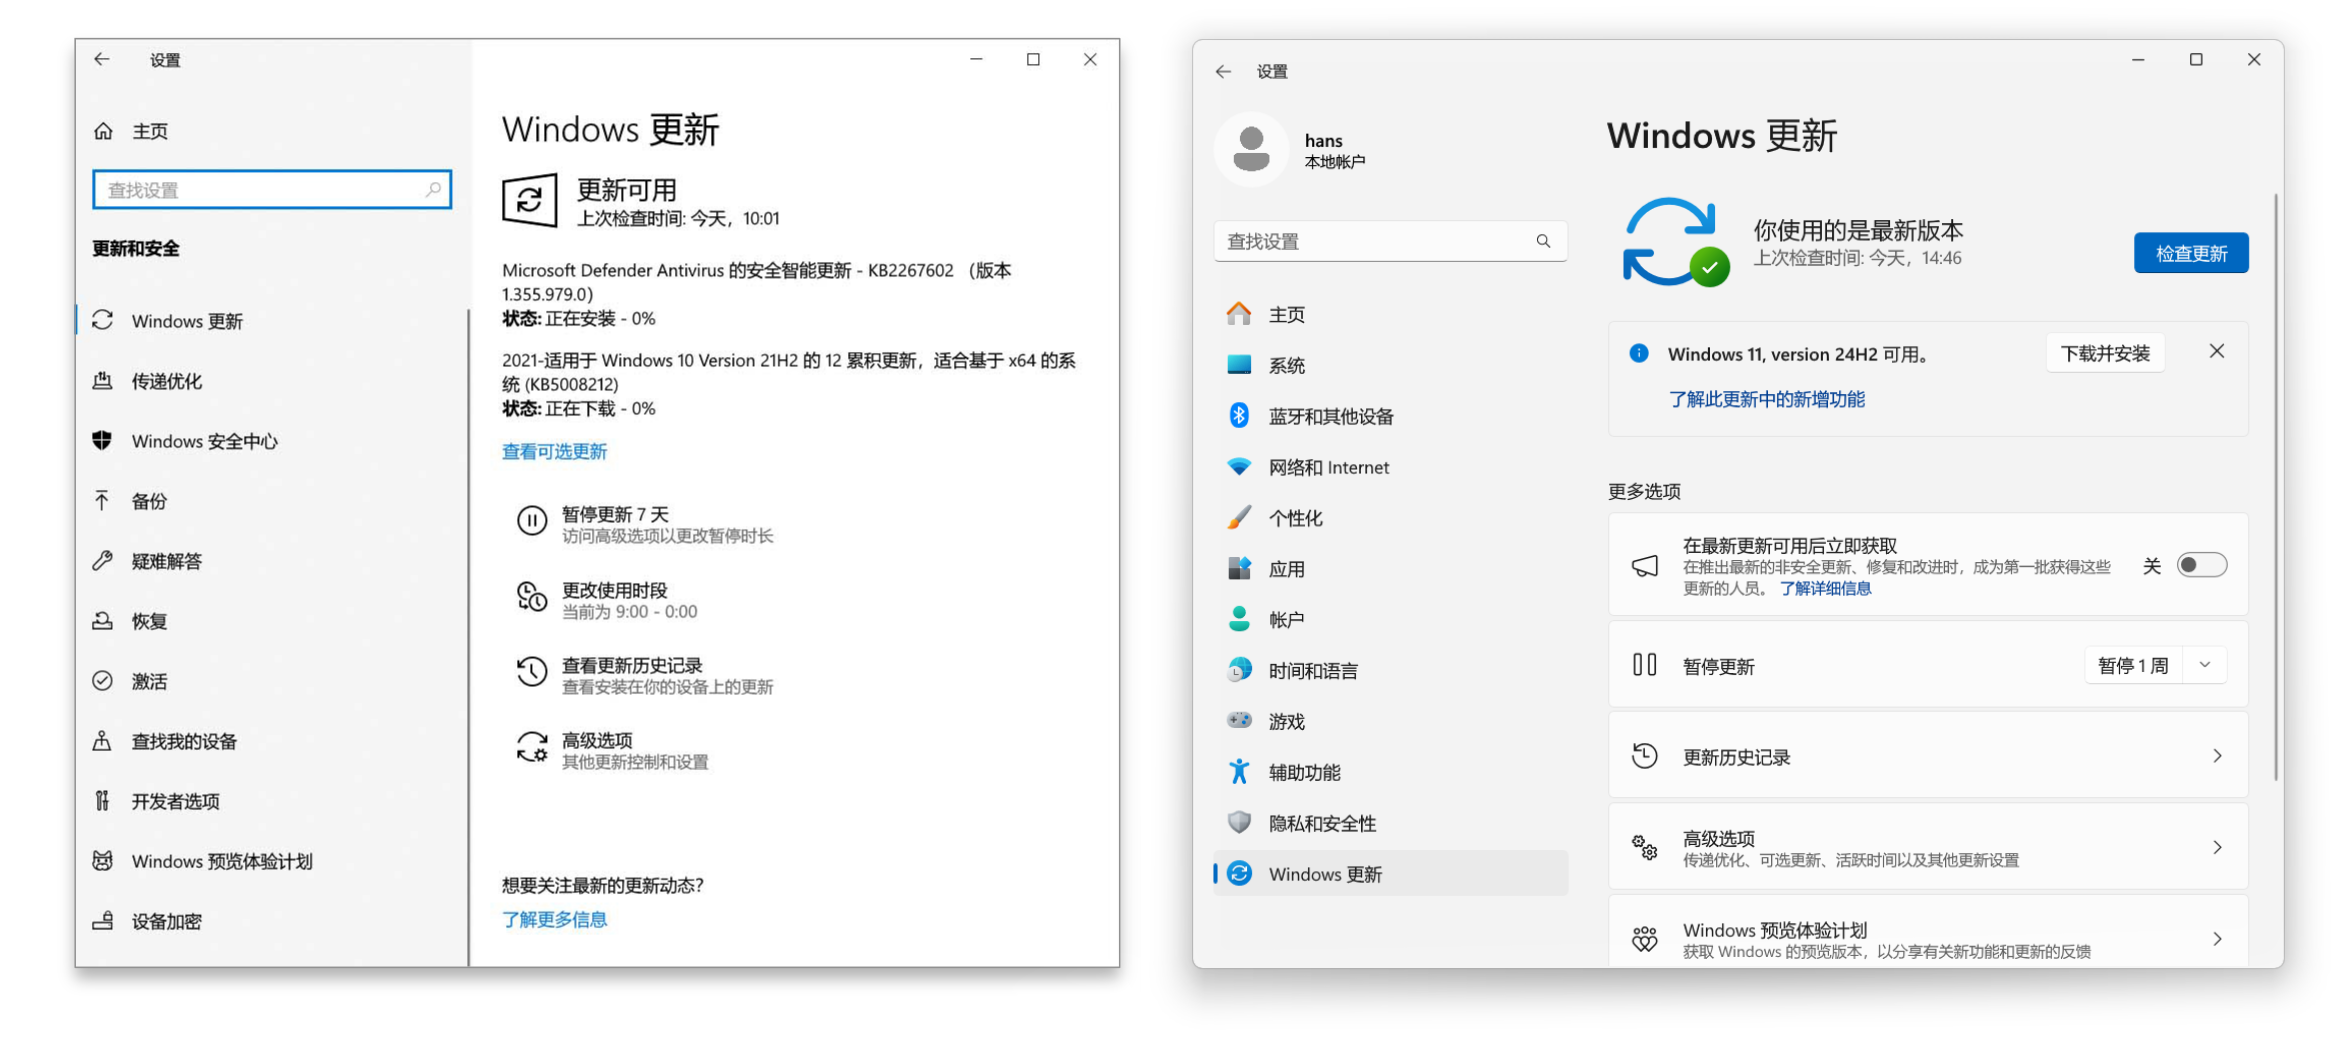
\includegraphics[width=.85\textwidth]{assets/basic/Update.png}
  \caption{Windows 10 (左)与 Windows 11(右)的「Windows 更新」界面}
  \label{Windows_Update}
\end{figure}

在今天的 Windows 系统中,Windows 更新主要会包括以下这些内容:

\begin{itemize}
  \item Windows 系统本身的补丁。其中包括一些对系统高危安全漏洞的「修补」,是微软给 Windows 中存在的安全问题的补丁。
  \item 电脑驱动程序的更新。这保证了你电脑上运行的驱动程序是最新的,(理论上)能更好地发挥电脑的性能。
  \item 电脑的「体验更新」。这是一些最直观的更新,主要包括系统外观与体验的优化。相比上面两项,这些更新更加容易被我们感知。
\end{itemize}

这样看来,Windows 更新应该是一件人见人爱的美事,但事实并非如此。除了阻碍我们关机睡觉之外,Windows 更新还存在一定风险——那些第一晚跑 Windows 更新,然后第二早电脑就无法启动的「翻车」事件已是屡见不鲜。事实上,Windows 更新和我们手机的「系统更新」本质一样,都会触碰系统最核心的部分。如果这个过程中出了一些差错,就可能让系统损坏,轻则功能不正常,重则完全无法启动。

但我们不至于因噎废食,而且还是基本上噎不着的情况下。事实上,那些因为 Windows 更新导致系统损坏的情况,大都是因为用户在电脑更新时手动打断,而非 Windows 更新自身的问题。Windows 更新提供了大量的系统安全补丁和更新,它们对保护系统安全的意义相当重大。所以,仅仅为了可能因不当操作损坏电脑就禁用 Windows 更新并不是理智的做法,况且,现在完全关闭 Windows 更新的步骤也挺复杂。

因此,我们所需要做的,就是正确对待 Windows 更新。保证 Windows 更新的安全的最重要前提,就是\regcolor{不要打断 Windows 更新}。事实上,在系统更新的过程中,屏幕上就会一直提示你「请不要断开电源」。在 Windows 更新进行的过程中,我们强烈建议将电脑(包括笔记本电脑,即使它内部装有电池,即使电池是充满电的)始终连接到交流电源,同时也不要盖上笔记本的盖子,为的是让系统「不受打扰」地完成整个更新流程。

\section{远离恶意软件}

所谓恶意软件,就是指那些诱导用户下载、安装其他软件,传染性强,且难以卸载的软件,大家都叫它们「流氓软件」。在上一章最后,我们亲眼见证了在恶意软件横行的年代,一个不干净的「高速下载器」捆绑安装的一大群软件。这个「高速下载器」就是典型的恶意软件,它所安装的这些软件中有不少更是恶意软件。恶意软件具有传染性,即一个恶意软件可能捆绑安装 5 个恶意软件,而这 5 个则可以捆绑更多同类(真是「一生二,二生三,三生万物」啊)。最后落得的,就是一台被「玩坏了」的电脑(实验过程中,并没有任何真实电脑遭受伤害):

\begin{figure}[htb!]
  \centering
  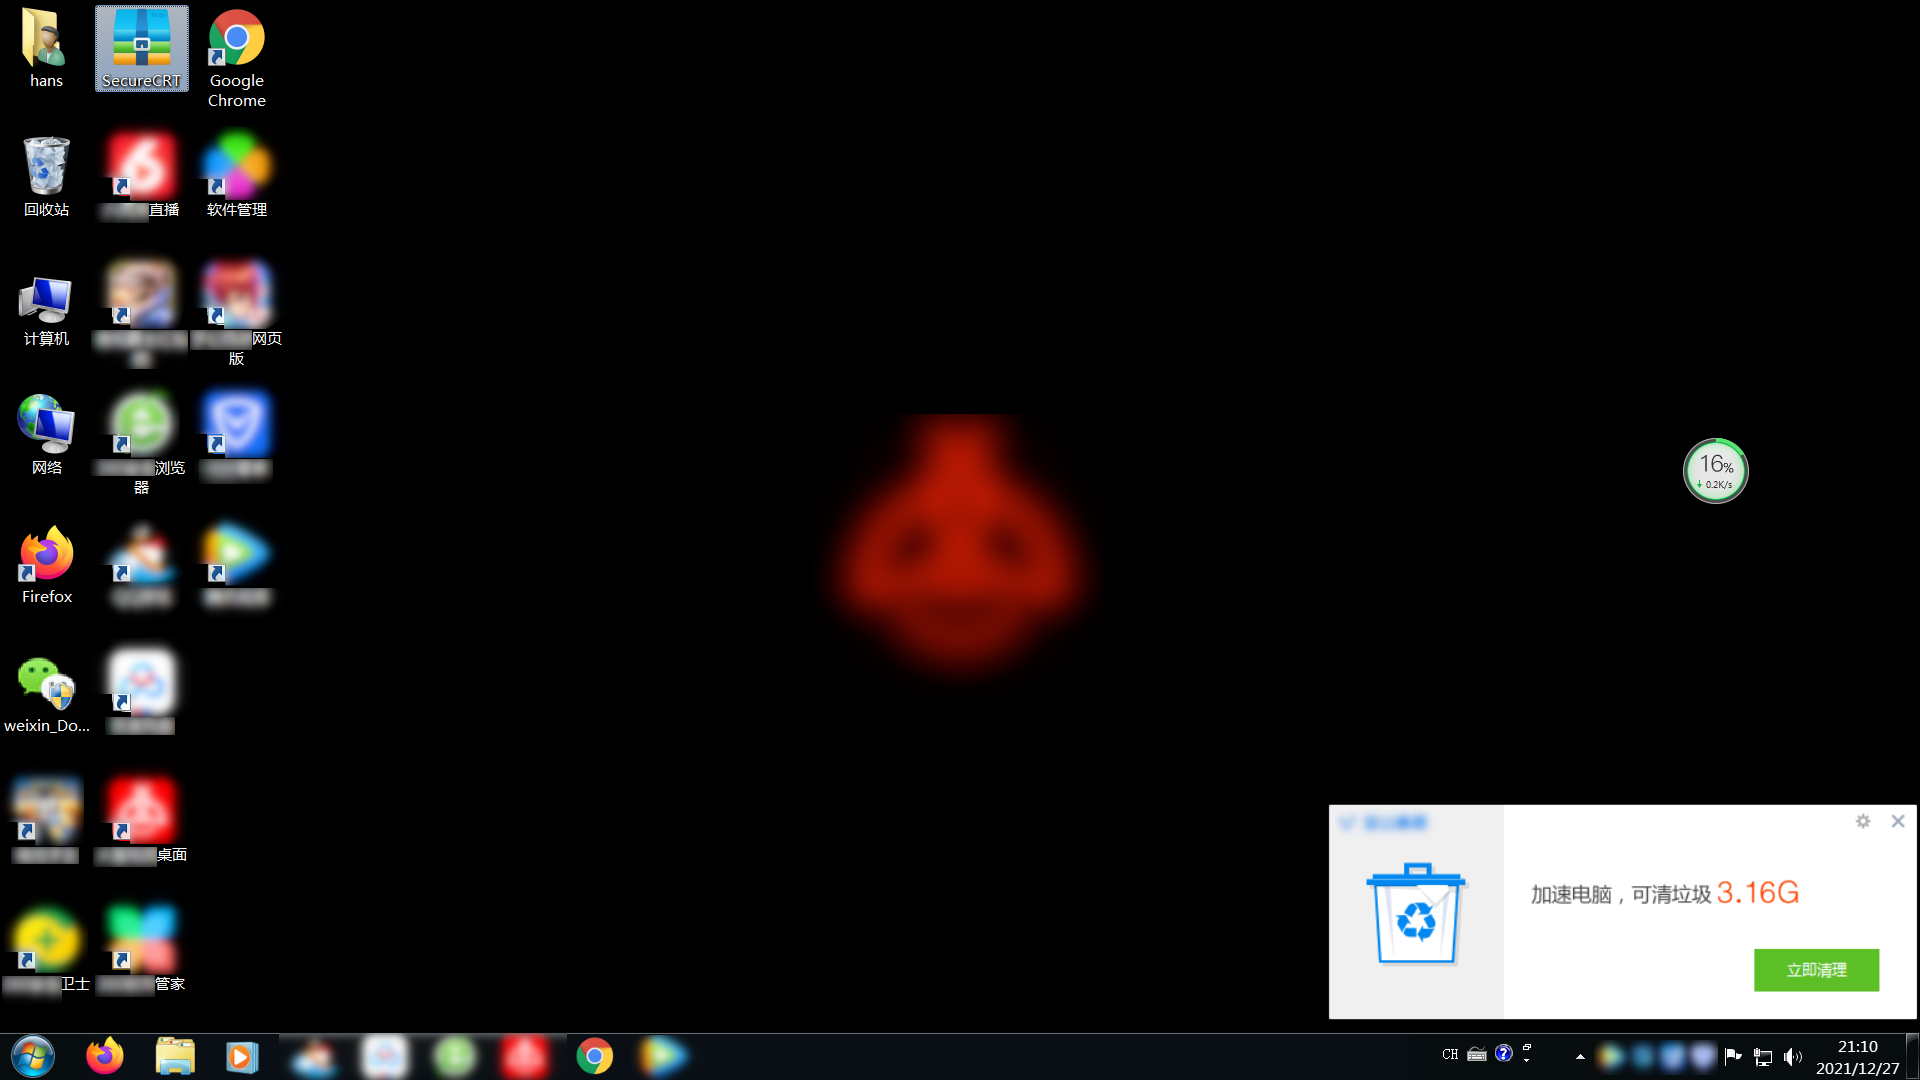
\includegraphics[width=.8\textwidth]{assets/basic/Computer_with_unwanted_software.png}
  \caption{被「玩坏了」的电脑}
  \label{fig:Computer_with_unwanted_software2}
\end{figure}

\begin{dangerbox}
  \centering
  远离恶意软件!\par
  \large 远离恶意软件!\par
  \LARGE 远离恶意软件!\par
\end{dangerbox}

如果你在电脑上发现了莫名其妙出现的软件,请卸载它们。一般情况下,对这些软件使用正常的卸载流程就能完成卸载。但\regcolor{特别注意卸载时的捆绑勾选}。然而有些时候,部分恶意软件会出现「卸载后卷土重来」的情况,这是因为它的安装被一个上级软件控制着,使得你的电脑在联网时会自动安装恶意软件。此时,不妨想想最近是否为一些奇怪的软件赋予了特殊权限,然后找出上级软件,优先卸载,再去卸载其他恶意软件。

下面列出了一些软件。在多次实验中,我们发现它们很容易被恶意软件捆绑安装。如果你在不知情的情况下,发现电脑上突然被安装这些软件,就要开始警惕了——建议卸载它们并对电脑上所有安装的软件进行排查。

\begin{itemize}
  \item 「2345」家族,包括「2345 浏览器」「2345 好压」「2345 电脑管家」「2345 看图王」等一系列软件。
  \item 「快压」「巧压」「微压」「布丁压缩」「52 好压」等一批压缩工具。
  \item 「飞速 PDF」「小树 PDF」「熊猫 PDF」「极光 PDF」等一批 PDF 查看器。
  \item 「新速头条」等资讯类弹窗软件。
  \item 「小黑记事本」等小工具类软件。
  \item 「布丁桌面」「海螺桌面」「火萤视频桌面」等「桌面」类软件。
  \item 「手机模拟大师」「Steam 游戏助手」「Steam 管家」「傲视霸主」等游戏类软件。
\end{itemize}

清单总是有限的,但互联网上的软件是无穷多的。一言以蔽之,一旦你电脑上突然冒出来非你主动安装的软件,请立即卸载并检查电脑上安装的软件清单。\CJKsout*{(不会吧不会吧,不会有人自己去装恶意软件吧。)}

\section{警惕「电信诈骗」}

众所周知,现在勒索病毒横行,染上之后任谁都束手无策。如果你没安装什么危险软件,但某天在上网时,电脑突然弹出了这样的「对话框」,你的第一反应是什么呢?

\begin{figure}[htb!]
  \centering
  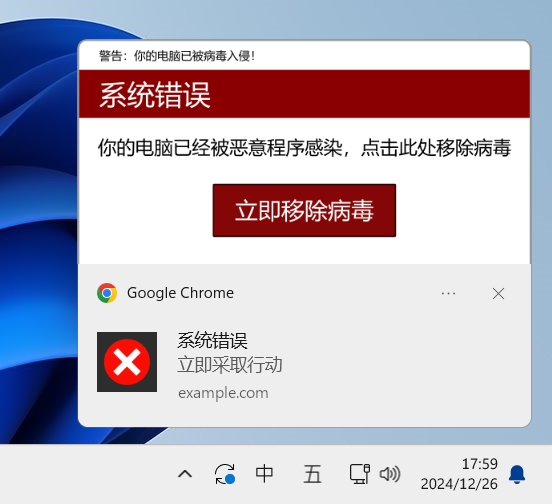
\includegraphics[width=.5\textwidth]{assets/basic/Fake_anti_virus_notification.png}
  \caption{可疑的「对话框」}
  \label{fig:Fake_anti_virus_notification}
\end{figure}

尽管这个「对话框」看起来像是系统弹出的警报,但它实际上是 Chrome 浏览器发出的一个\regcolor{网页通知}。就像手机上的许多应用可以在屏幕顶部弹出通知一样,浏览器中打开的网页也可以在电脑上发送通知。仔细观察这个通知,我们会发现,它包含了一张伪造成弹窗的图片,以及一个伪造成系统警告的图标。通过巧妙利用 Windows 通知的展示方式,这个通知成功以假乱真,让人误以为它来自系统本身。

\begin{figure}[htb!]
  \centering
  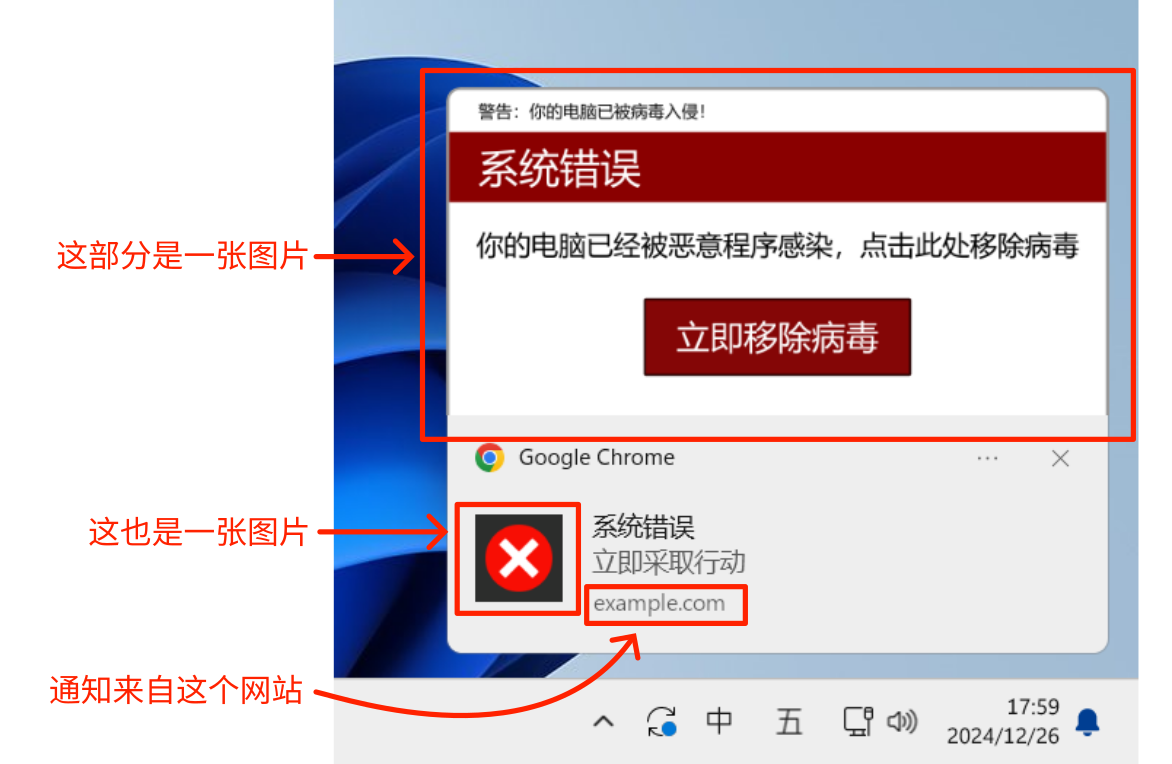
\includegraphics[width=.65\textwidth]{assets/basic/Fake_notification_components.png}
  \caption{「对话框」的真实组成}
  \label{fig:Fake_notification_components}
\end{figure}

这种通知称为「\regcolor{恶意浏览器通知}」,本质是一种「\regcolor{电信诈骗}」。\regcolor{如果我们点击了这个通知的任何位置,就会打开一个含有恶意软件或代码的网站},直接进了对方的圈套。除了这个例子中展示的「你的电脑含有病毒」外,类似的电信诈骗还包括「你的支付账户已经泄露」「你涉嫌违法已被起诉」等等。由于这样的「对话框」往往能伪造得以假乱真,我们很容易就被它欺骗,从而造成严重的后果。

如何鉴别这种电信诈骗通知呢?首先,几乎所有浏览器在网站要求发送通知时,都会明确询问用户是否接收该网站的通知,如下图所示。显然,除了那些包含邮件、聊天功能的动态网站外,我们不应该随意允许其他网站发送通知。这样就能从根本上减少遭遇这种电信诈骗的可能性。

\begin{figure}[htb!]
  \centering
  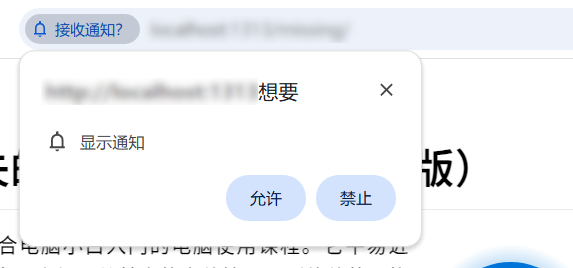
\includegraphics[width=.55\textwidth]{assets/basic/Website_ask_for_notification_permission.png}
  \caption{浏览器正在请求通知}
  \label{fig:Website_ask_for_notification_permission}
\end{figure}

其次,当电脑上弹出任何可疑的窗口时,我们都要保持警惕——在点击它们之前,先想一想:这个窗口是由什么软件产生的?为什么它会弹出?仔细观察,我们可以找到一些蛛丝马迹:在上述例子中,我们可以看到窗口中有「Google Chrome」字样。作为一个浏览器,Chrome 本身绝不会弹出类似「电脑中存在病毒」这样的警告信息。同时,当我们遇到「你的支付账户泄露」甚至是「你涉嫌违法」时,都应当仔细思考一下——银行或警方真的会用这样的方式来通告我们吗?相信在思考之后,我们就能很容易地得出结论——选择将弹出通知的网站关闭。

实际上,除了这种「恶意浏览器通知」式的电信诈骗,还有一些恶意网站通过强制网页全屏显示伪造的窗口,同样通过「电脑病毒」「账户泄露」「你有违法行为」等恐吓性信息,来让用户乖乖交钱。我们只需要学会\regcolor{保持冷静,理性分析,识别出嫌疑网站并将之关闭},就能有效防止自己遭受真正的损失。

\begin{note}
  有些恶意网站会采用「推送服务」机制,能让你即使没有打开对应的网站,也能接收来自它们的通知。如果要关闭这种通知,你可以在网上搜索「\texttt{<浏览器名字>} 关闭网站通知」。
\end{note}

\practice

\begin{enumerate}
  \item 在\autoref{fig:Uninstalling_1} 所示的界面中,按哪个按钮可以卸载?
  \item 在\autoref{fig:Uninstalling_2} 所示的界面中,按哪个按钮可以卸载?
  \item 在\autoref{fig:Uninstalling_3} 所示的界面中,按哪个按钮可以卸载?
  \item 在\autoref{fig:Uninstalling_4} 所示的界面中,如何操作可以卸载?
    \begin{figure}[htb!]
      \centering
      \begin{minipage}{.44\textwidth}
        \centering
        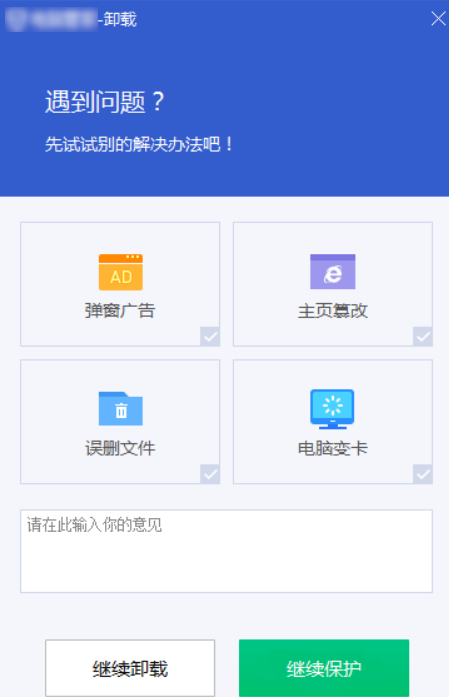
\includegraphics[width=.95\textwidth]{assets/basic/Uninstalling_1.png}
        \caption{第1题图}
        \label{fig:Uninstalling_1}
      \end{minipage}
      \begin{minipage}{.55\textwidth}
        \centering
        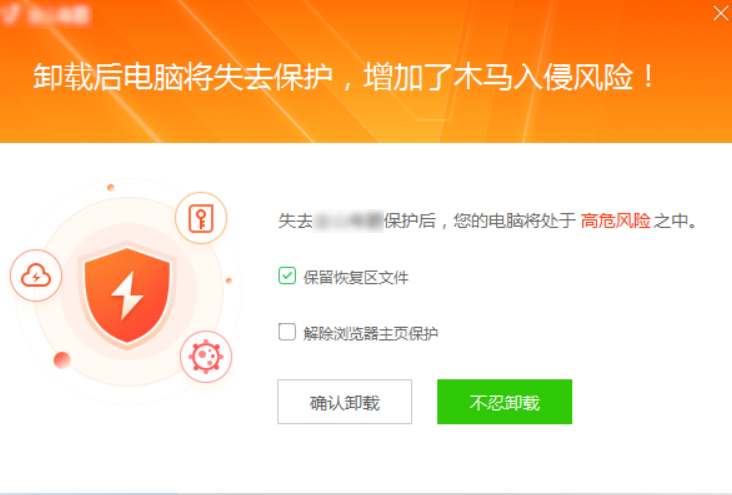
\includegraphics[width=.9\textwidth]{assets/basic/Uninstalling_2.png}
        \caption{第2题图}
        \label{fig:Uninstalling_2}
        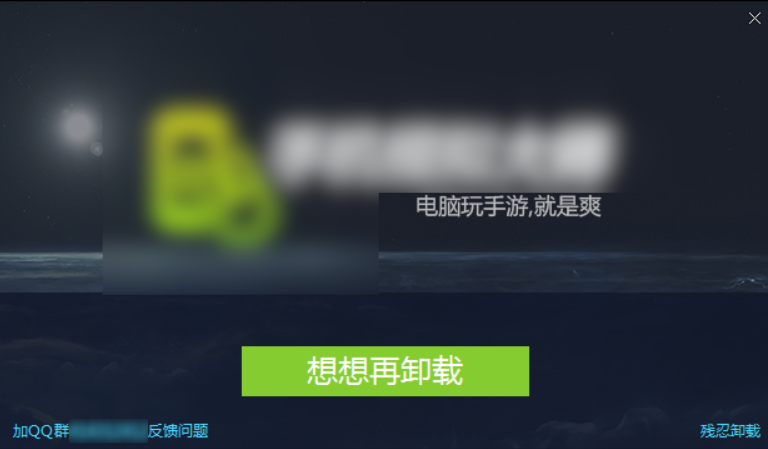
\includegraphics[width=.95\textwidth]{assets/basic/Uninstalling_3.png}
        \caption{第3题图}
        \label{fig:Uninstalling_3}
      \end{minipage}
      \\
      \begin{minipage}{.6\textwidth}
        \centering
        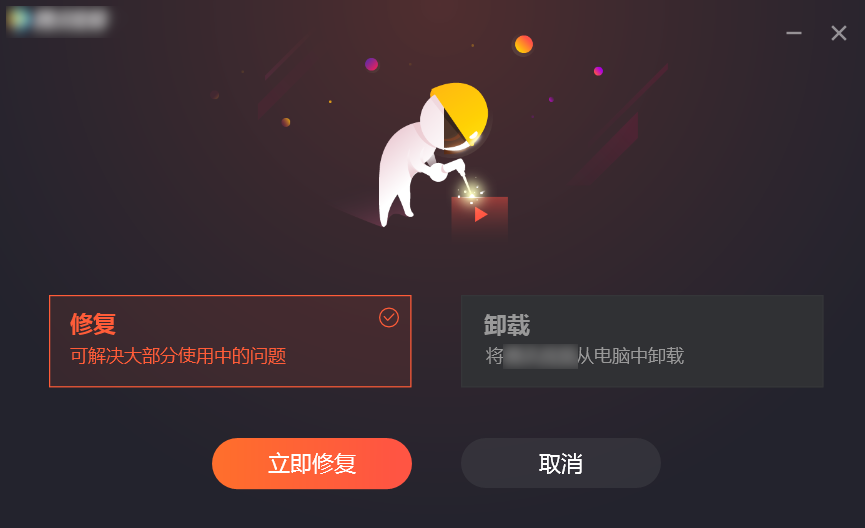
\includegraphics[width=.95\textwidth]{assets/basic/Uninstalling_4.png}
        \caption{第4题图}
        \label{fig:Uninstalling_4}
      \end{minipage}
    \end{figure}
  \item 清理电脑上的杀毒软件 / 安全软件,保留一个你用得最熟悉的。
\end{enumerate}